\chapter*{How to Get Fedora?}
\section*{Getting Fedora}

You can install Fedora from optical media (CD, DVD), a USB flash drive, or over the network by using an appropriate installation image. Installation images of \emph{Fedora~Workstation} are available for download in the ISO format at \url{getfedora.org}. \emph{Fedora Workstation} defaults to a 64-bit operating system download as that is what is best for most users.

If you aren't ready to install Fedora yet and would like to try it first without losing or changing anything already on your PC, make sure you download a live image. With this image, you can boot to a fully functional system and find out what Fedora is like, experiment with it, and determine whether it fully supports your PC's hardware.

To run \emph{Fedora Workstation} reasonably well it is recommend that you have at least a 1~GHz processor, 2~GiB of memory, 10~GiB of hard drive space, and a graphics card that supports hardware acceleration. These aren't the minimum requirements, but they are the best for most users. Some users may wish to run Fedora on lower powered machines and will find it performs well there too.

\section*{Creating Installation Media}

In order to install or run Fedora from an installation image, you need to create installation media first:
\begin{itemize}
\item\emph{USB Installation} -- To create a USB installation drive, you can use the \emph{Fedora Media Writer}. It can run on \emph{MS Windows}, \emph{Apple macOS} or Linux. Beware, this program will erase all the data on the flash drive! \emph{Fedora Media Writer} can download the installation image for you when you run it. If you're using \emph{MS Windows} or \emph{Apple macOS}, the installation file of the application is what you'll be offered when you decide to download \emph{Fedora Workstation} at \url{getfedora.org}.

\emph{GNOME and Disks} -- If you already use a Linux operating system with the GNOME desktop environment, you can use built-in software to write to a USB drive. In the \emph{Files} application, right-click an ISO image, choose \enquote{Open in a different app} and then choose \enquote{Write on disk}. This will open the \emph{Disks} utility which will write the image on to a flash drive.

If you decide to write the installation image on to a USB flash drive, carefully double-check that you've picked the correct target drive. If you're doing this on \emph{MS Windows}, you need to pick the character that has been assigned to the drive you'd like to use (typically this will be \texttt{D:} or \texttt{E:}). On Linux, you need to do the same using the device (typically this is will be \texttt{/dev/sdX} where \texttt{X} is an alphabetic character). The easiest and safest way to do this on Linux is to use the \emph{Disks} utility mentioned above.

\item\emph{DVD Installation} -- Using a \emph{DVD} is a very traditional way of installing Fedora. You can create an installation DVD by writing an ISO image to a DVD. Most modern operating systems can do this operation with built-in software. If not, you can install a specialized application such as \emph{Brasero} on Linux and \emph{ImgBurn} on \emph{MS Windows}. All versions of \emph{Apple macOS} can write DVDs using \emph{Finder} and \emph{Disk Utility}.
\end{itemize}

\section*{Installing Fedora}
\begin{enumerate}
\item\emph{Booting} -- No matter what media you've chosen, you'll need to make sure that you set the right boot sequence in the BIOS of the computer you'd like to install Fedora~Workstation on. The drive with the install media needs to be in the first position. You can get to the BIOS configuration by pressing a specific key after starting the computer. The key depends on the vendor (typically the keys are \keystroke{Delete}, \keystroke{F1}, or \keystroke{F2}). Alternately, many vendors allow you to choose a boot drive without having to go to the BIOS settings by pressing the \keystroke{F12} key.

\item\emph{Initial Screen} -- After successfully booting from the installation media, you'll see the initial screen where you can choose between installing Fedora~Workstation (or booting into the live system) and verifying the install media. If you choose installation, you'll boot into the live system and will be asked if you want to try the system out or install it on the hard drive. If you choose to \enquote{Try Fedora} you can use it in this way for as long as you want and can choose to perform an installation at any time by clicking on the installer icon in the menu.

\begin{figure}[ht]
\begin{center}
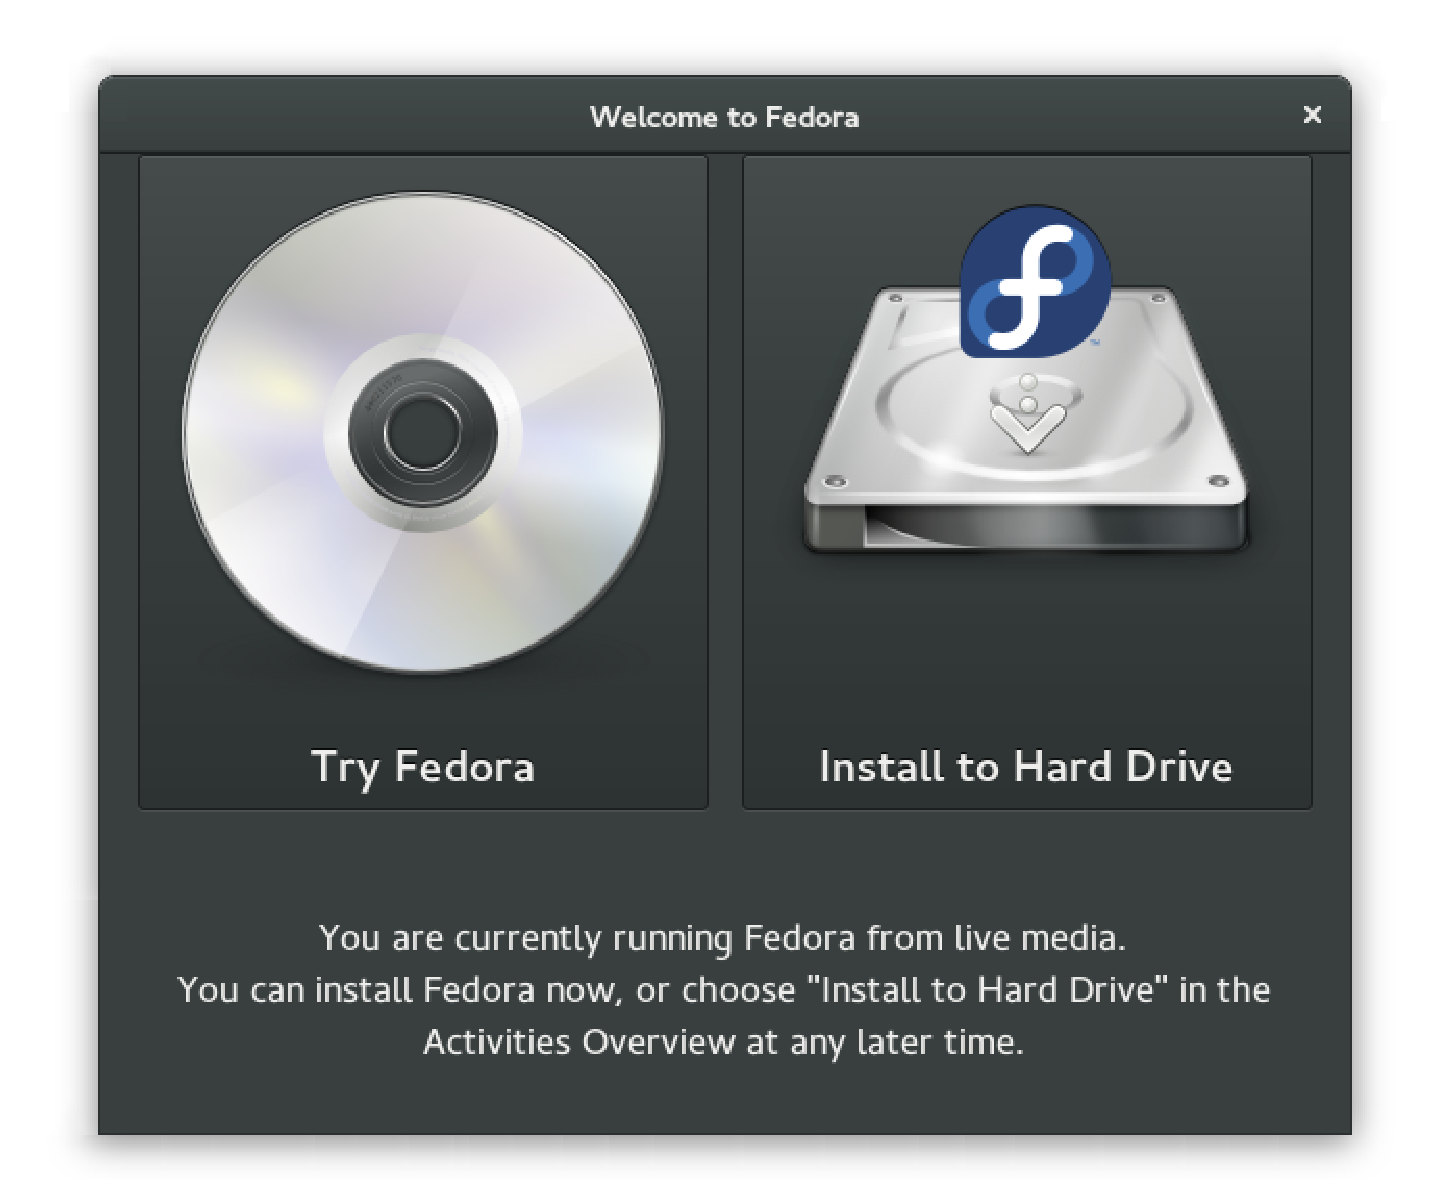
\includegraphics[width=.75\textwidth]{img/instalator-a}
\captionbelow{Booted installation media of Fedora Workstation} \label{fig:installer-a}
\end{center}
\end{figure}

\item\emph{Trying the System} -- If you've chosen to try the system, you'll begin using the \emph{GNOME~Shell}. The top of the display contains the most commonly used control elements. There is an \emph{Activities} button in the upper left corner which will get you to applications (and to the option to install Fedora Workstation on your system). The upper right corner has controls that allow you to set up the network, as well as to restart or shut down the system.

\item\emph{Installer} -- Once you decide to install Fedora Workstation, you'll being using the installation program, Anaconda. The installer consists of different spokes that manage the options for areas such as language settings, time zone, etc.

\begin{figure}[ht]
\begin{center}
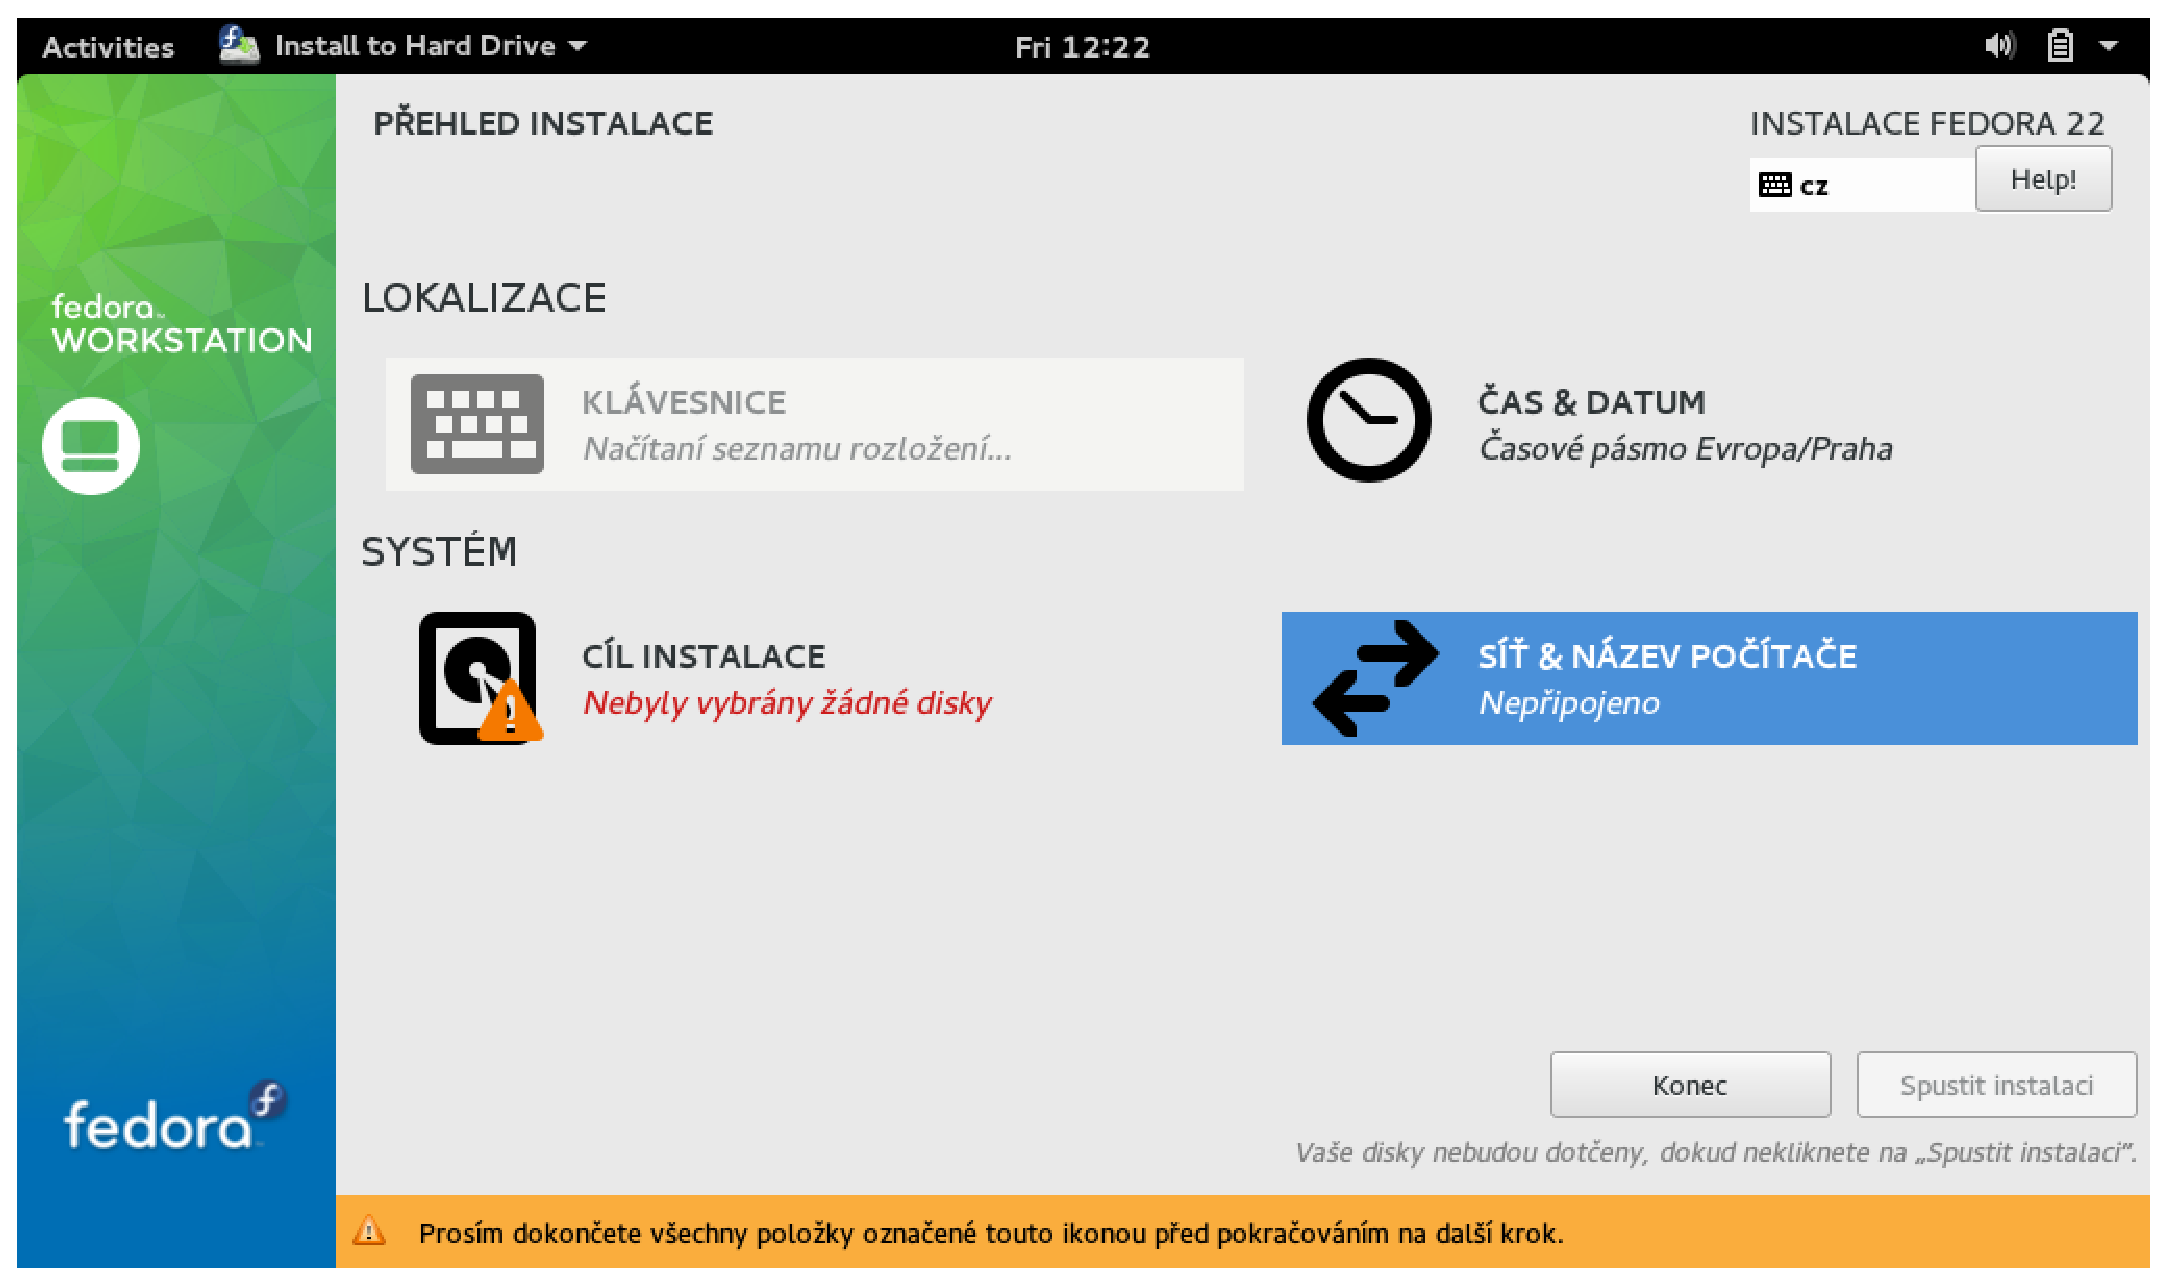
\includegraphics[width=0.95\textwidth]{img/installer-b}
\captionbelow{Fedora Workstation Installer} \label{fig:installer-b}
\end{center}
\end{figure}

The disk partitioning spoke is the most important part of the installer. This spoke will define where on your hard drive Fedora Workstation will be installed. The installer offers you automatic partitioning which will configure the hard drive in a way that is useful for most people, or you can also choose manual partitioning and apply a customized setting. It is also possible to set up encryption for better security.

Fedora Workstation also allows you to create a dualboot system, that is, to have two operating systems installed on your PC at the same time. It's easy to install Fedora Workstation next to an existing \emph{MS Windows} installation.

In the partitioning dialog, you will see the existing partitions on the left. Before you confirm the changes make sure that everything is the way you meant it to be (for example that all partitions of other operating systems are still there, if you wish to keep them). When you confirm the changes and start the installation, the changes will be final.

\item\emph{Finishing the Installation} -- While the system is being installed, you need to provide several important pieces of information such as the root or administrator password and the information for creating a user account.

You will normally use the user account you created and only use the root password when you need to make a system-wide change. Fedora Workstation has the classic approach to user accounts where the root account is not disabled. However, if you do not want to remember passwords for two accounts, you can check the \emph{Admin} option when creating your user account. This enables the account to act as an administrator in vast majority of operations and avoids your having to use the root password often.
\end{enumerate}

And that's it. The whole installation should take less than several dozen minutes. After a restart you'll just need to perform a couple of short post-install tasks such as changing the boot order to the original state and then you're ready to go.

Everything worked well? Now you can start exploring Fedora Workstation!

\endinput
